\clearpage
%
\chapter{Electron Identification}
\label{cha:eID}
%
Electrons are identified by putting each negative track for a given event through a series of nine cuts.
A candidate electron is considered a ``good'' electron only if it passes all nine cuts.
If an event has more than one good electron, the highest momentum one is chosen.
The nine cuts, described in detail in the subsequent sections, are: matching cuts on the $\theta$ and $\phi$ angles in the CC, a $\theta$ vs $\phi$ fiducial cut, a momentum dependent cut on the EC energy, a cut on the energy in the inner EC, a geometric cut on the EC, fiducial cuts on regions 1 and 3 of the DC, and a cut on the z vertex.
%

\section{CC $\theta$ Matching}
\label{sec:CCthetaMatching}
%
Due to the geometry of the CC, the correspondence between polar angle in the CC, $\theta_{CC}$, and the CC segment number for scattered electrons is manifestly surjective.
A cut is therefore applied on $\theta_{CC}$ for each segment of the CC by fitting the $\theta_{CC}$ distribution with a gaussian plus a polynomial background; events within 3$\sigma$ of the mean pass the cut, see figure~\ref{fig:CCseg_c1}.
%
\begin{figure}[htp]
\centering
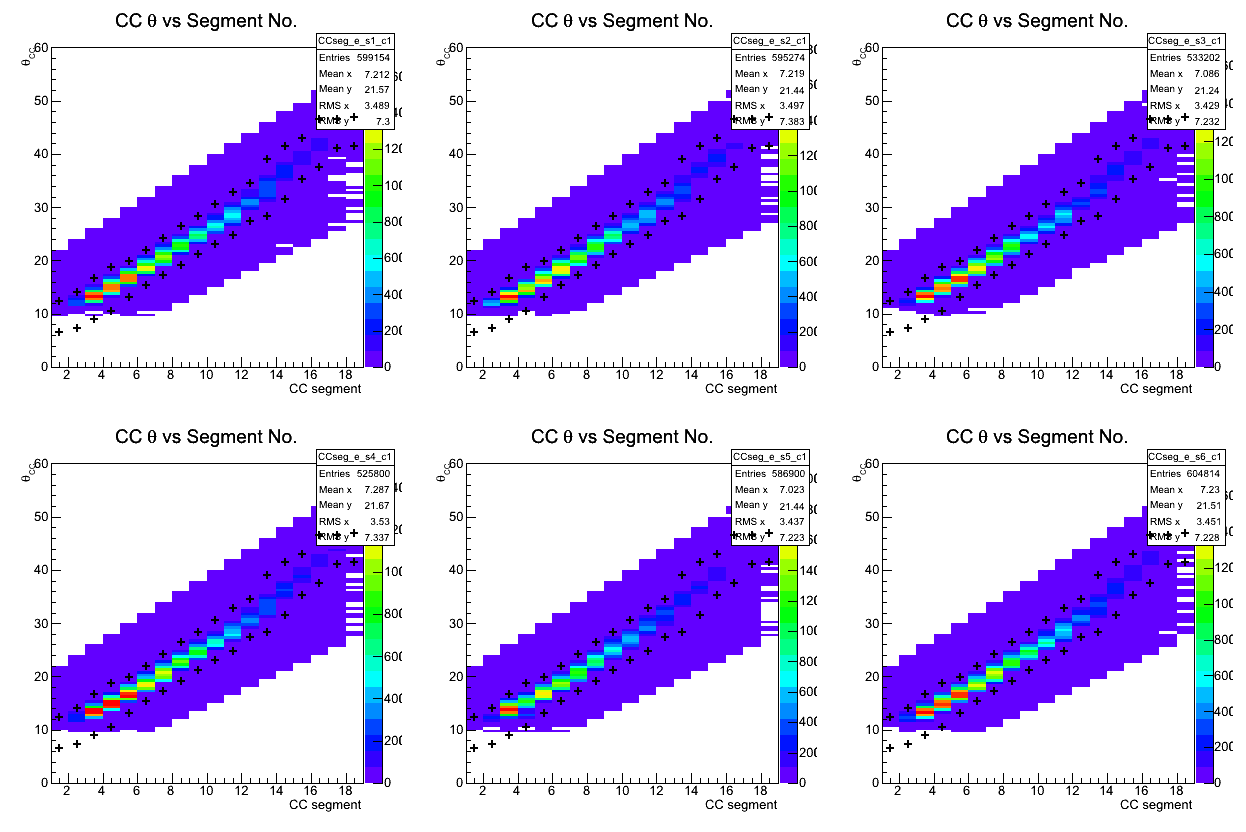
\includegraphics[width=5in]{figures/CCseg_c1.png}
\caption{$\theta_{CC}$ vs CC segment number for each of the six sectors of CLAS. These plots already have the other eight cuts applied and the current cut is given by the black crosses.}
\label{fig:CCseg_c1}
\end{figure}
%
%
\section{CC $\phi$ Matching}
\label{sec:CCphiMatching}
%
Each sector of the CC is divided in half such that each side is a mirror image of the other.
If a track is on one side of the sector but the PMT that fired was on the other side, then the event was likely background and not a good event.
A CC $\phi$ matching algorithm is used that returns 0 if both PMTs fire, $\pm$1 if the track and PMT are on the same side, and $\pm$2 if the track and PMT are on opposite sides.
Events that return $\pm$2 are rejected, all other events are kept.
See figures~\ref{fig:CCphiMatch_c0}~and~\ref{fig:CCphiMatch_c1}.
%
\begin{figure}[htp]
\centering
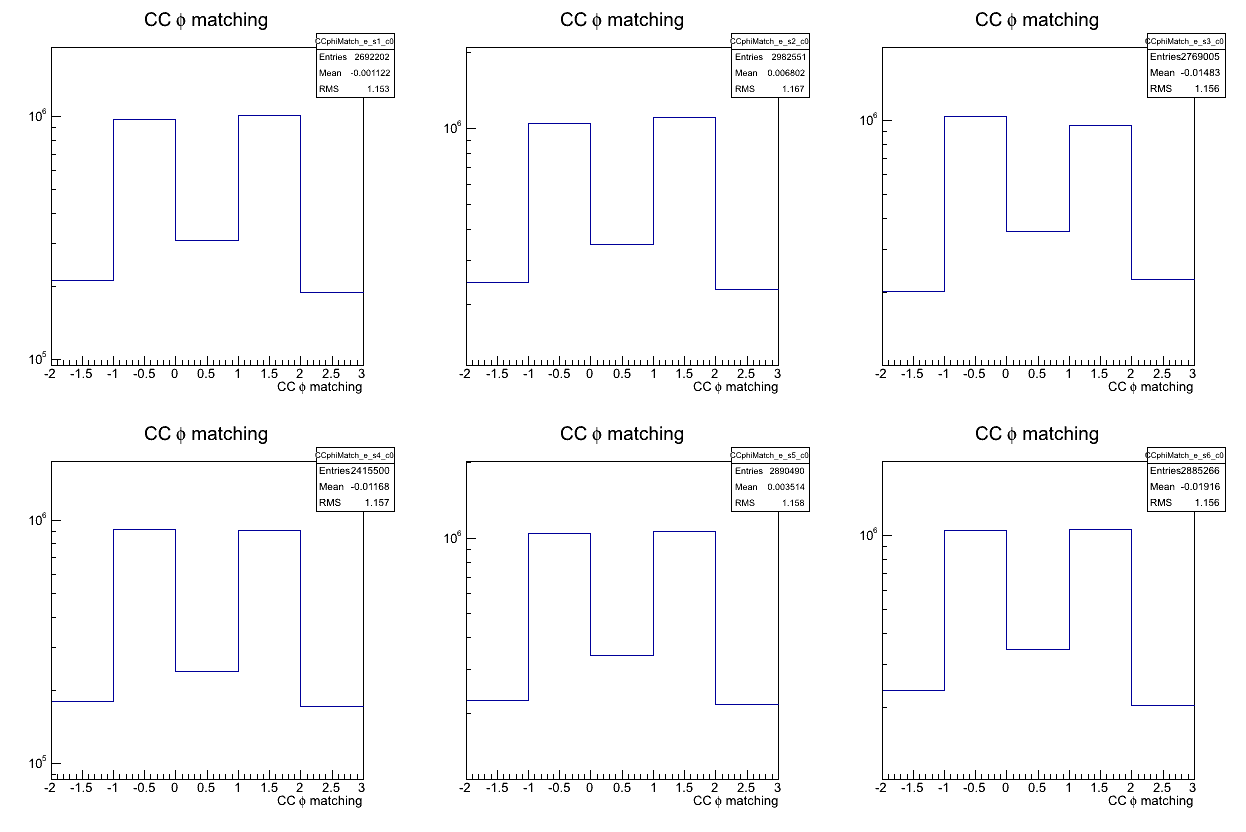
\includegraphics[width=5in]{figures/CCphiMatch_c0.png}
\caption{CC $\phi$ matching distribution for negative tracks for each sector. The matching algorithm returns 0 if both PMTs fire, $\pm$1 if the track and PMT are on the same side, and $\pm$2 if the track and PMT are on opposite sides.}
\label{fig:CCphiMatch_c0}
\end{figure}
%
\begin{figure}[htp]
\centering
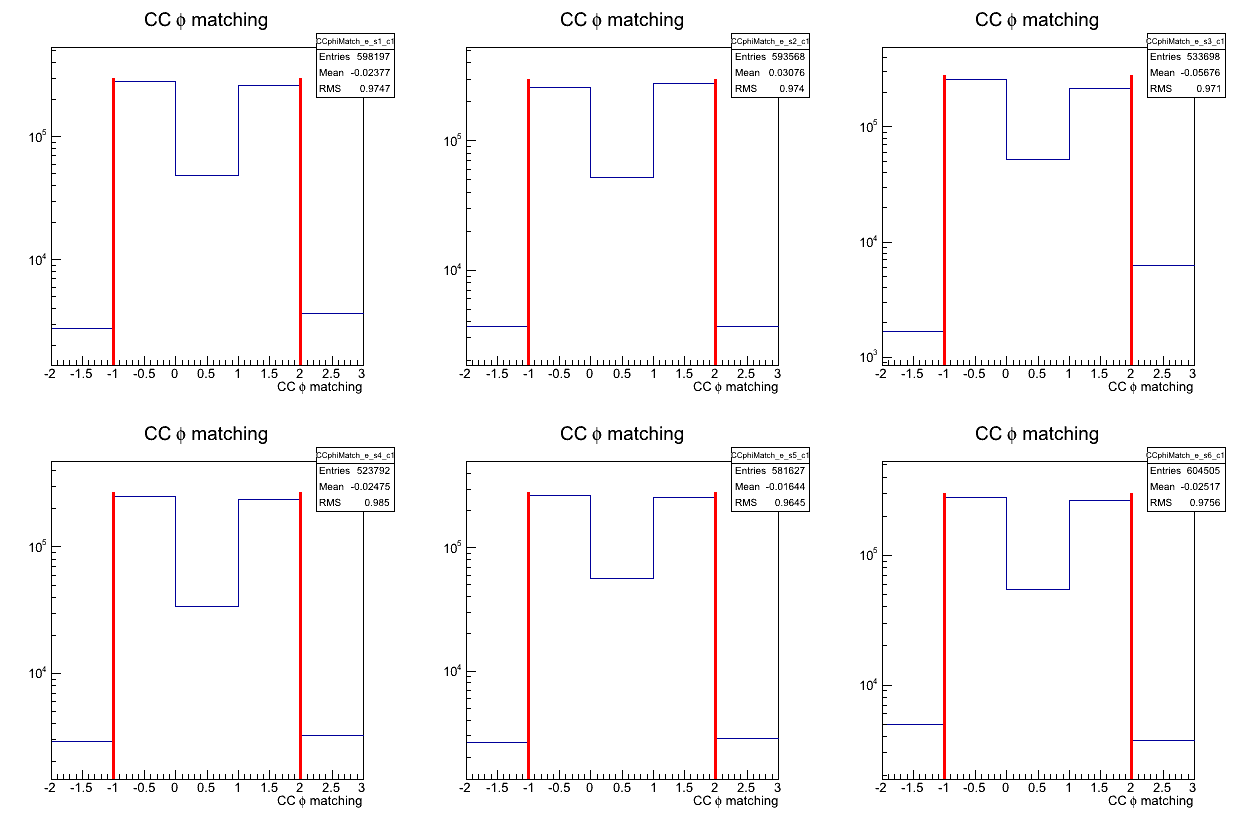
\includegraphics[width=5in]{figures/CCphiMatch_c1.png}
\caption{CC $\phi$ matching distribution for electron candidates with all other electron ID cuts applied for each sector. This cut is shown in red and removes candidate electrons for which the PMT and track are on opposite sides of the sector.}
\label{fig:CCphiMatch_c1}
\end{figure}
%
%
\section{CC Fiducial Cut}
\label{sec:CCfiducial}
%
A geometric cut of the form $\theta_{CC} > 46.0 - 35\sqrt{1 - \frac{\phi^{2}}{350}}$ (units of degrees) is applied to the CC.
The equation was obtained empirically based on the $\theta_{CC}$ vs $\phi$ (lab angle) distribution with and without other electron ID cuts applied.
%See figures~\ref{fig:CCfid_c0}~and~\ref{fig:CCfid_c1}.
See figure~\ref{fig:CCfid_c0c1_6sects}.
%
\begin{sidewaysfigure}[htp]
\centering
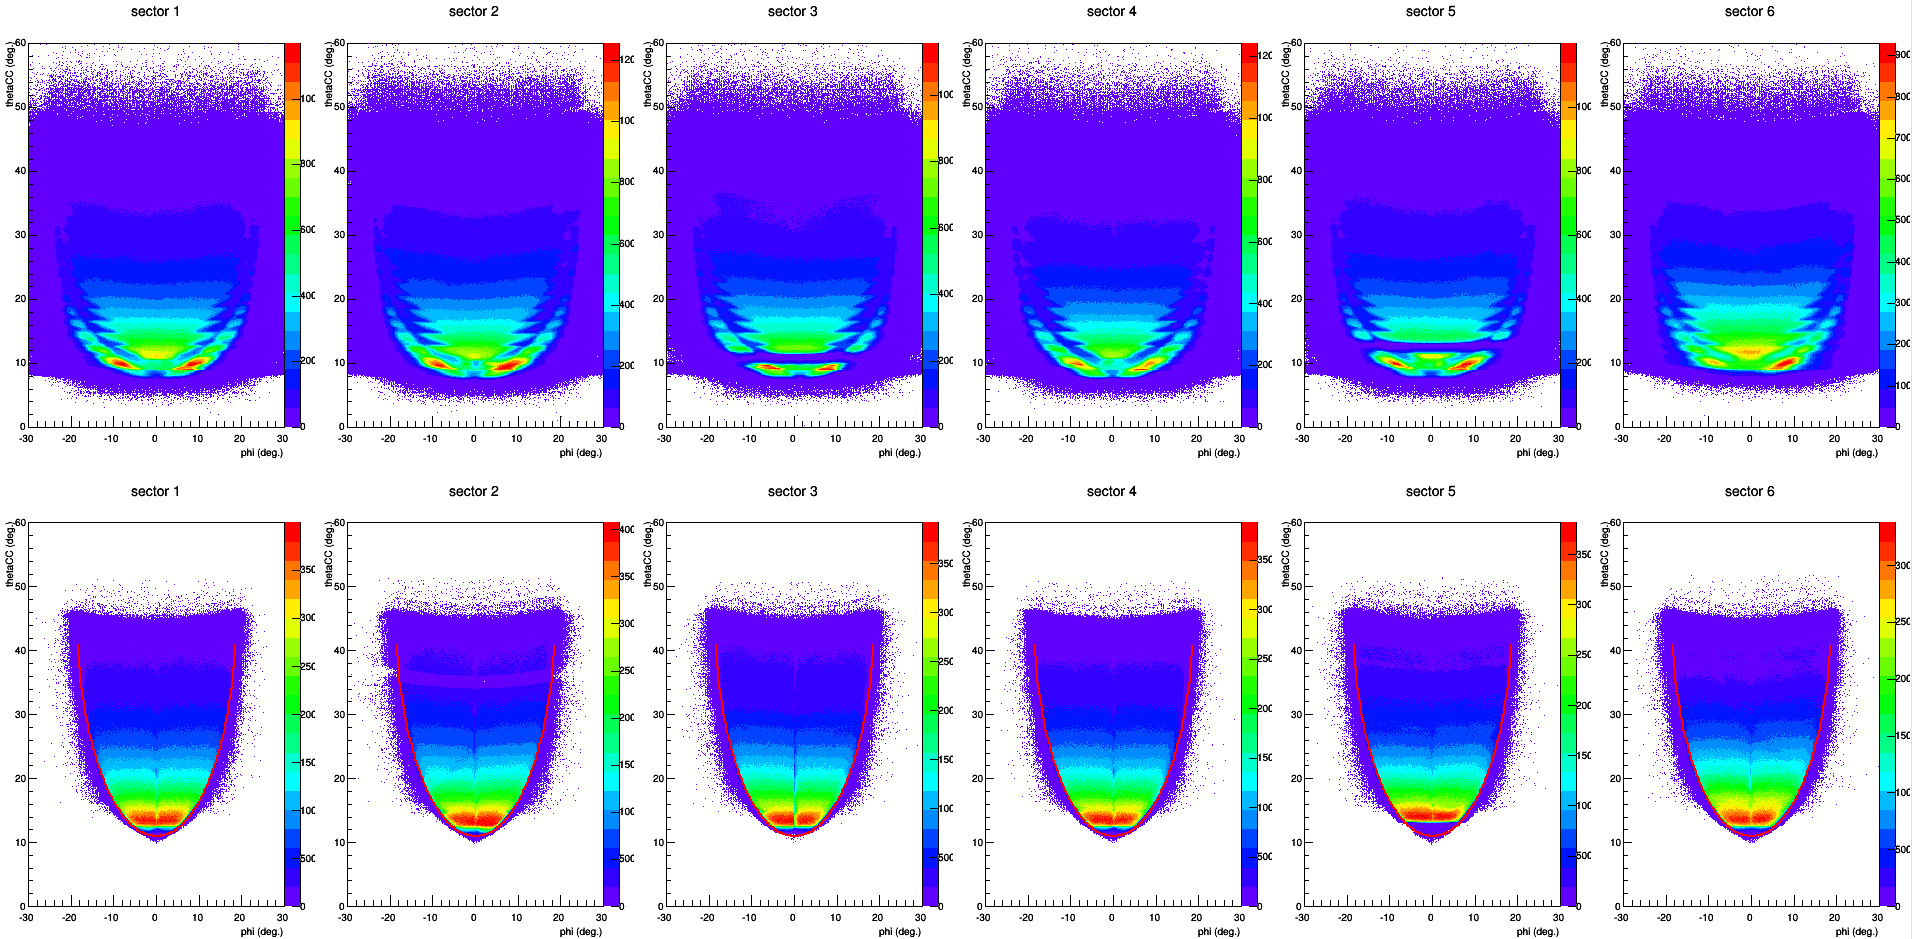
\includegraphics[width=8.5in]{figures/CCfid_c0c1_6sects.png}
\caption{$\theta_{CC}$ vs $\phi$ (lab angle) for each of the six CLAS sectors. The top row shows all negative tracks and the bottom row shows negative tracks which pass all the other electron ID cuts with this cut shown in red.}
\label{fig:CCfid_c0c1_6sects}
\end{sidewaysfigure}
%
%
\section{EC $E_{in}$ vs $E_{out}$ Cut}
\label{sec:ECinvsout}
%
The EC can be used to separate negatively charged pions from electrons in several ways.
Firstly, the scattered electron always travels in a forward direction while pions can have any direction; since the EC only covers forward angles, any track not producing a signal in the EC is immediately rejected.
Secondly, any pion over 0.5 GeV is minimum ionizing in the EC and produces less light in the PMTs than electrons do.
Therefore, only candidate electrons with an energy in the inner part of the EC greater than 0.06 GeV are kept (see figure~\ref{fig:ECoutVinPlot}).
%
\begin{figure}[htp]
\centering
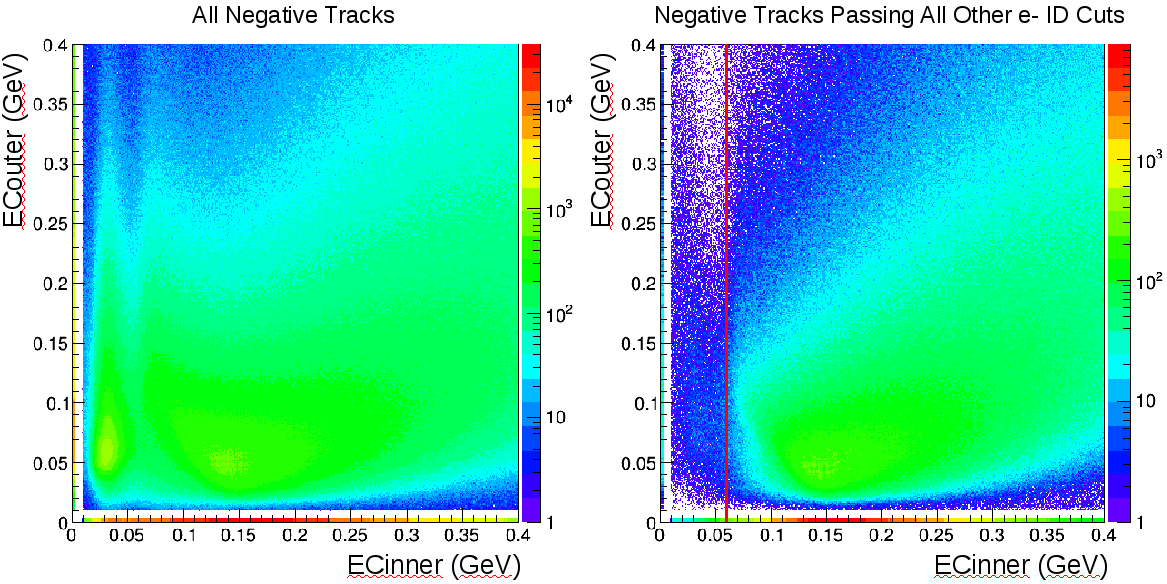
\includegraphics[width=6in]{figures/ECoutVinPlot.png}
\caption{outer EC energy vs inner EC energy plots for (left) all negative tracks and (right) negative tracks passing all other electron ID cuts. Tracks with and inner EC energy greater than 0.06 GeV pass this cut (shown by the red line in the plot on the right).}
\label{fig:ECoutVinPlot}
\end{figure}
%
\section{EC Sampling Fraction Cut}
\label{sec:ECsampling}
%
The ratio of total energy to momentum stays nearly constant as a function of momentum for electrons.
To eliminate background as well as contamination from other negative tracks, each momentum bin is fit with a gaussian and the points at $\mu + 5\sigma$ and $\mu - 3\sigma$ are fit with a second order polynomial to define the cut.
Figure~\ref{fig:ECsampling_c0c1_6sects} shows the E/p vs p distribution candidate electrons along with the cut described here.
%
\begin{sidewaysfigure}[htp]
\centering
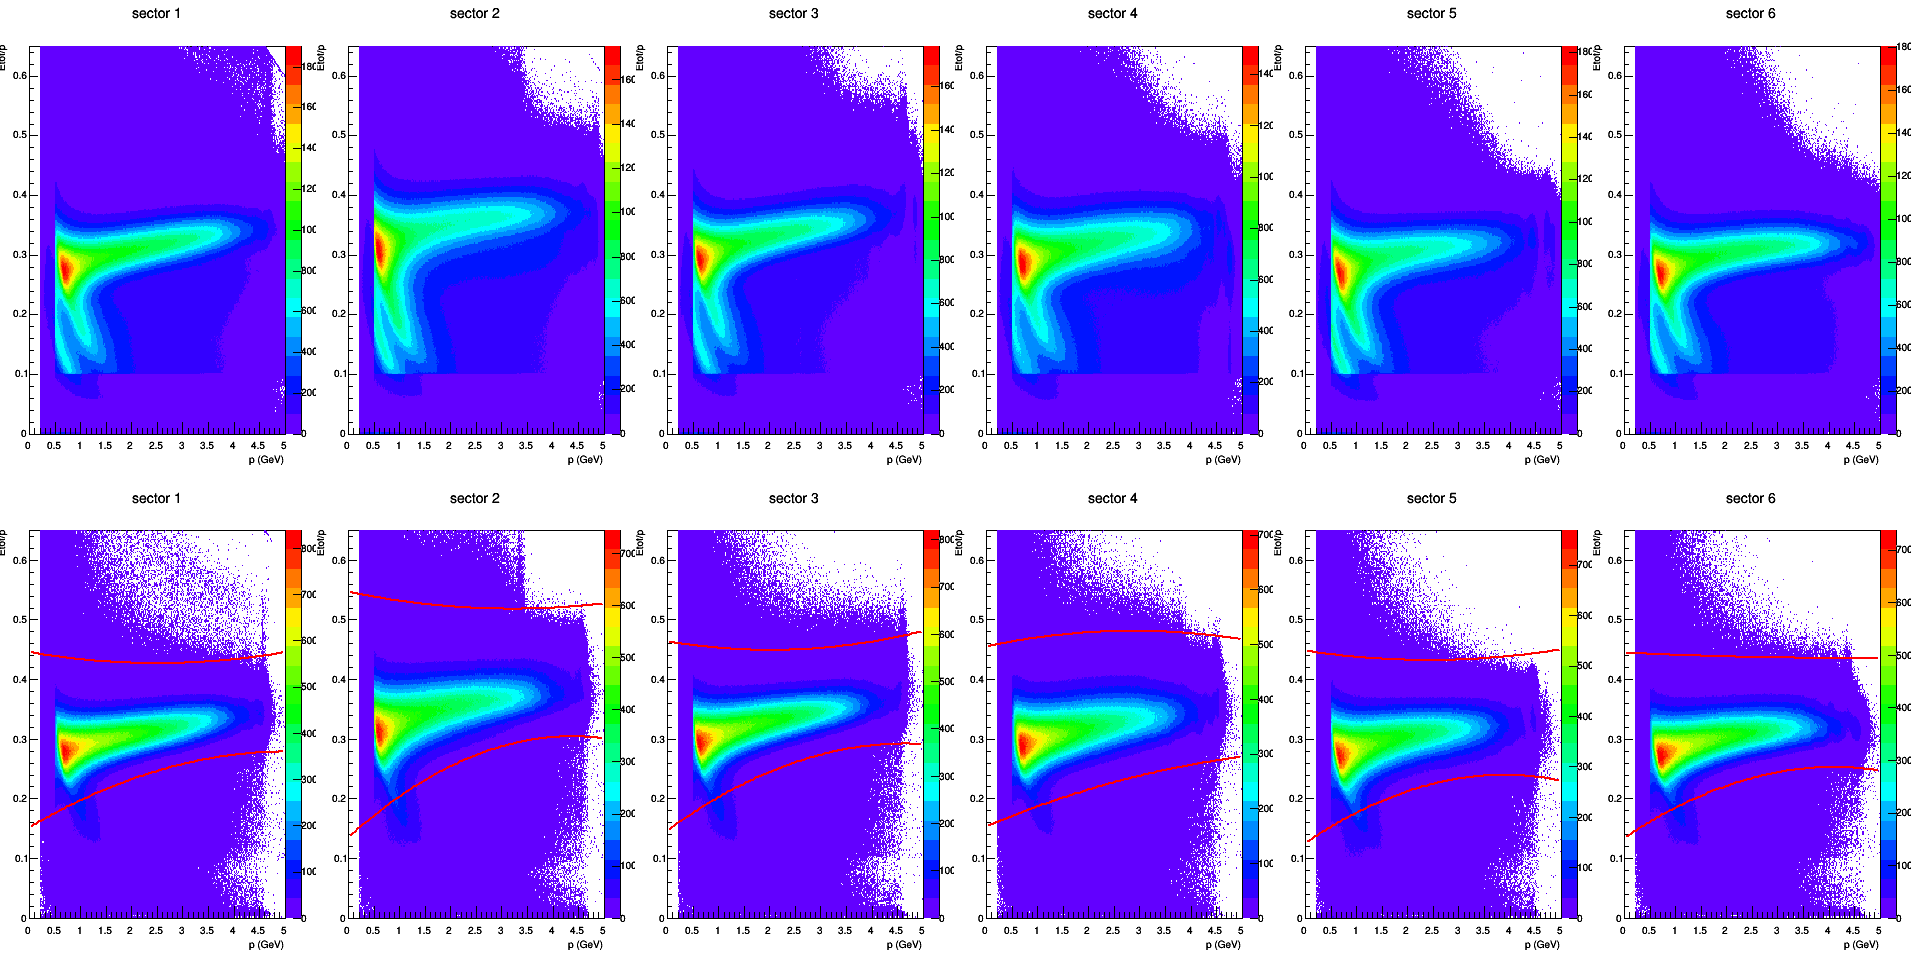
\includegraphics[width=8.5in]{figures/ECsampling_c0c1_6sects.png}
\caption{The energy deposited in the EC divided by momentum as a function of momentum for electron candidates for each of the six CLAS sectors. The top row shows all negative tracks and the bottom row shows the tracks passing all other electron ID cuts with this cut shown in red.}
\label{fig:ECsampling_c0c1_6sects}
\end{sidewaysfigure}
%
%
\section{EC Geometric Cut}
\label{sec:ECgeometric}
%
When a particle deposits its energy in the EC a ``shower'' is created.
If this shower occurs close to the edge of one of the EC triangles only a fraction of the particle's energy is reconstructed.
Since energy information about these particles is unreliable they are cut via a geometric cut on the EC (see figure~\ref{fig:ECgeometricPlot}).
%
\begin{figure}[htp]
\centering
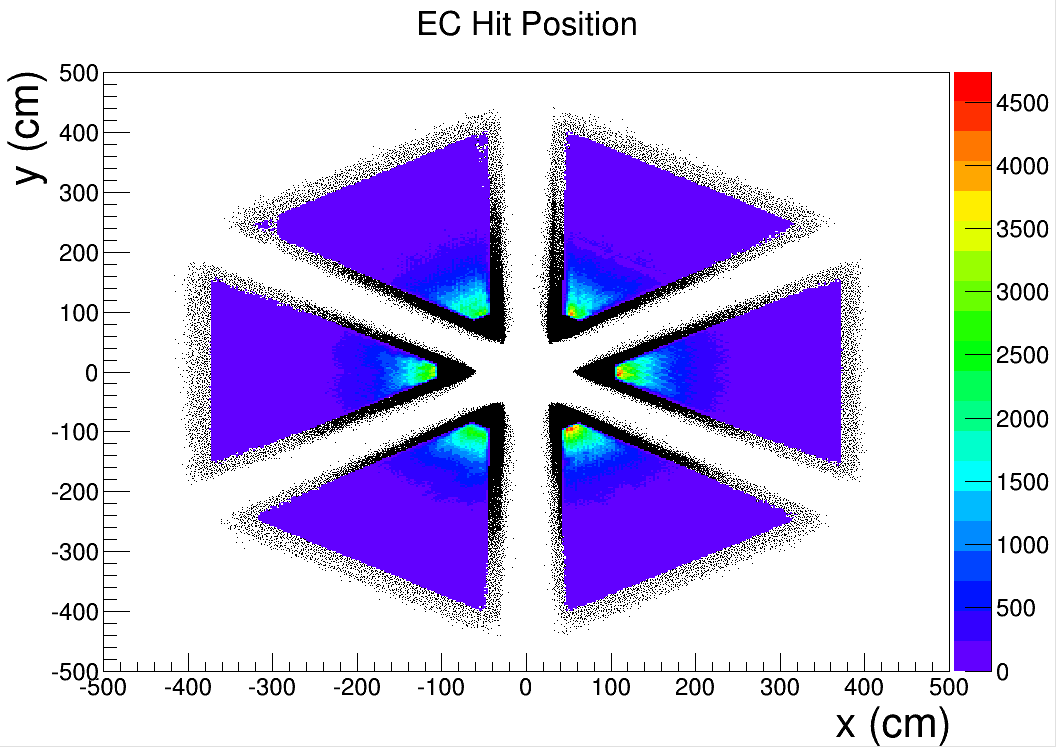
\includegraphics[width=5in]{figures/ECgeometricPlot.png}
\caption{The distribution of hits in the EC. The black points show the hit positions for all negative tracks and the colored points show the hit positions for the final electron sample. It can clearly be seen that tracks hitting near any of the edges have been removed.}
\label{fig:ECgeometricPlot}
\end{figure}
%
%
\section{Region 1 Fiducial Cut}
\label{sec:R1fid}
%
A geometric fiducial cut is applied to X-Y position of tracks in region 1 of the DC.
The cut is shown with red lines in figure~\ref{fig:R1fid_c0c1_6sects}.
The lines are symmetric about Y=0, form a $60^\circ$ angle, and intersect at X=22 cm.
These cuts were chosen to approximately respect the geometry of the DC.
%
\begin{sidewaysfigure}[htp]
\centering
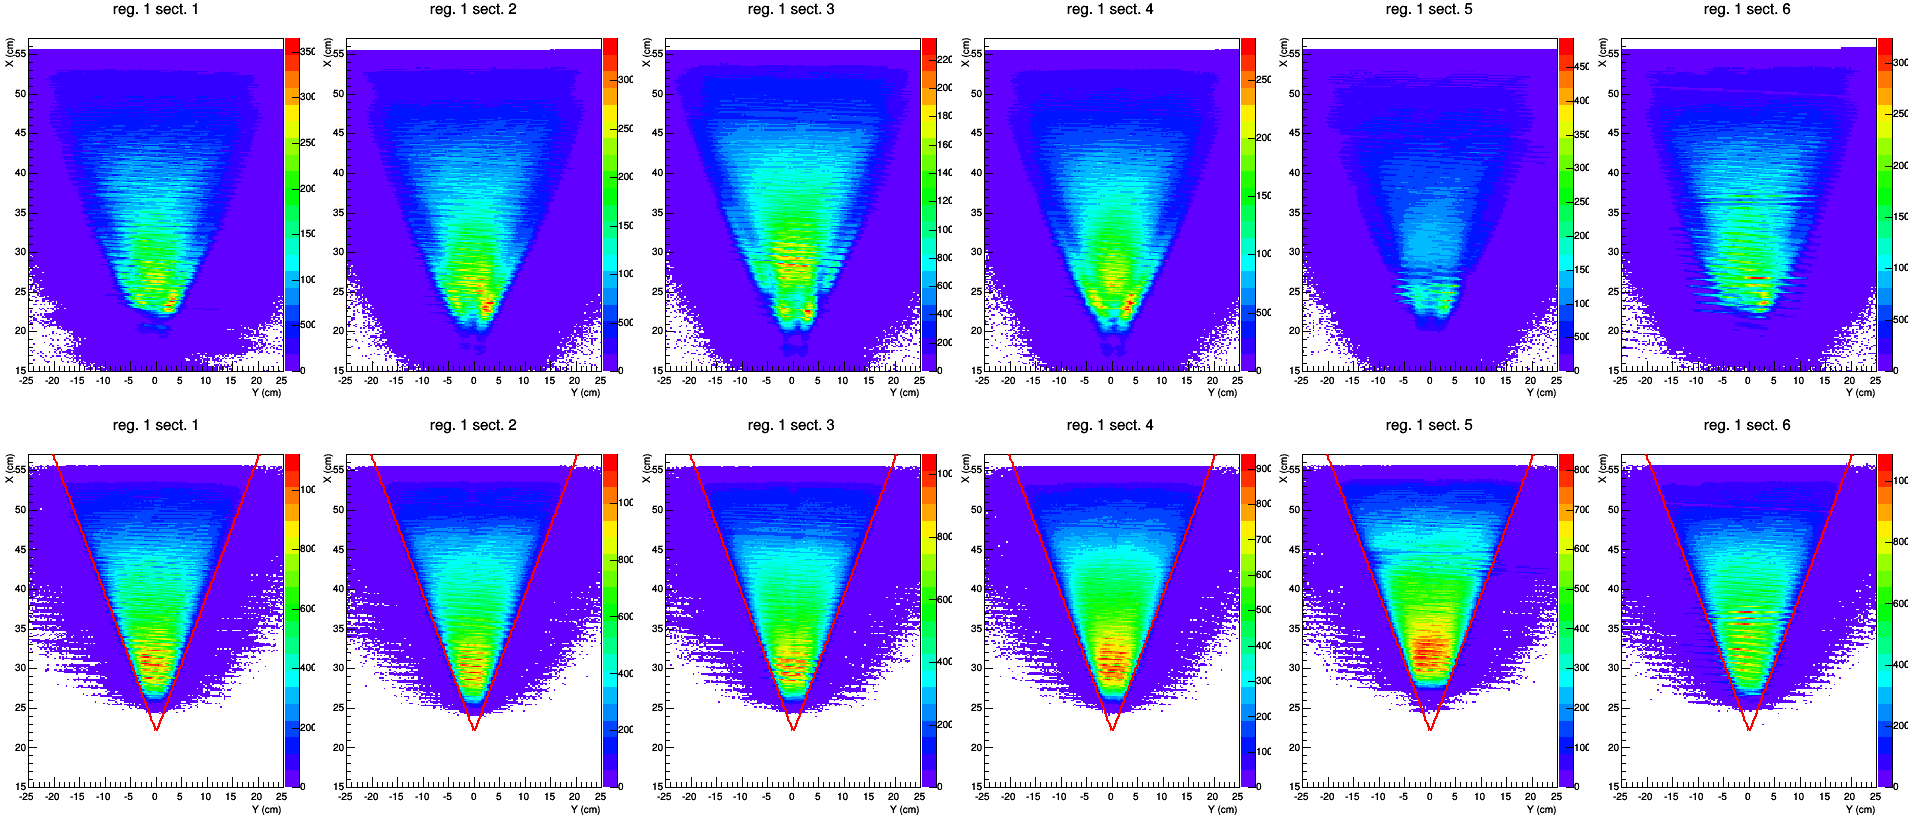
\includegraphics[width=8.5in]{figures/R1fid_c0c1_6sects.png}
\caption{The X vs Y position of tracks in region 1 of the DC for each sector. The top row shows results for all negative tracks and the bottom row shows results with all the other electron ID cuts applied. The cut applied here is shown with red lines.}
\label{fig:R1fid_c0c1_6sects}
\end{sidewaysfigure}
%
%
\section{Region 3 Fiducial Cut}
\label{sec:R3fid}
%
A geometric fiducial cut is applied to X-Y position of tracks in region 3 of the DC.
The cut is shown with red lines in figure~\ref{fig:R3fid_c0c1_6sects}.
The lines are symmetric about Y=0, form a $49^\circ$ angle, and intersect at X=83 cm.
These cuts were chosen to approximately respect the geometry of the DC.
%
\begin{sidewaysfigure}[htp]
\centering
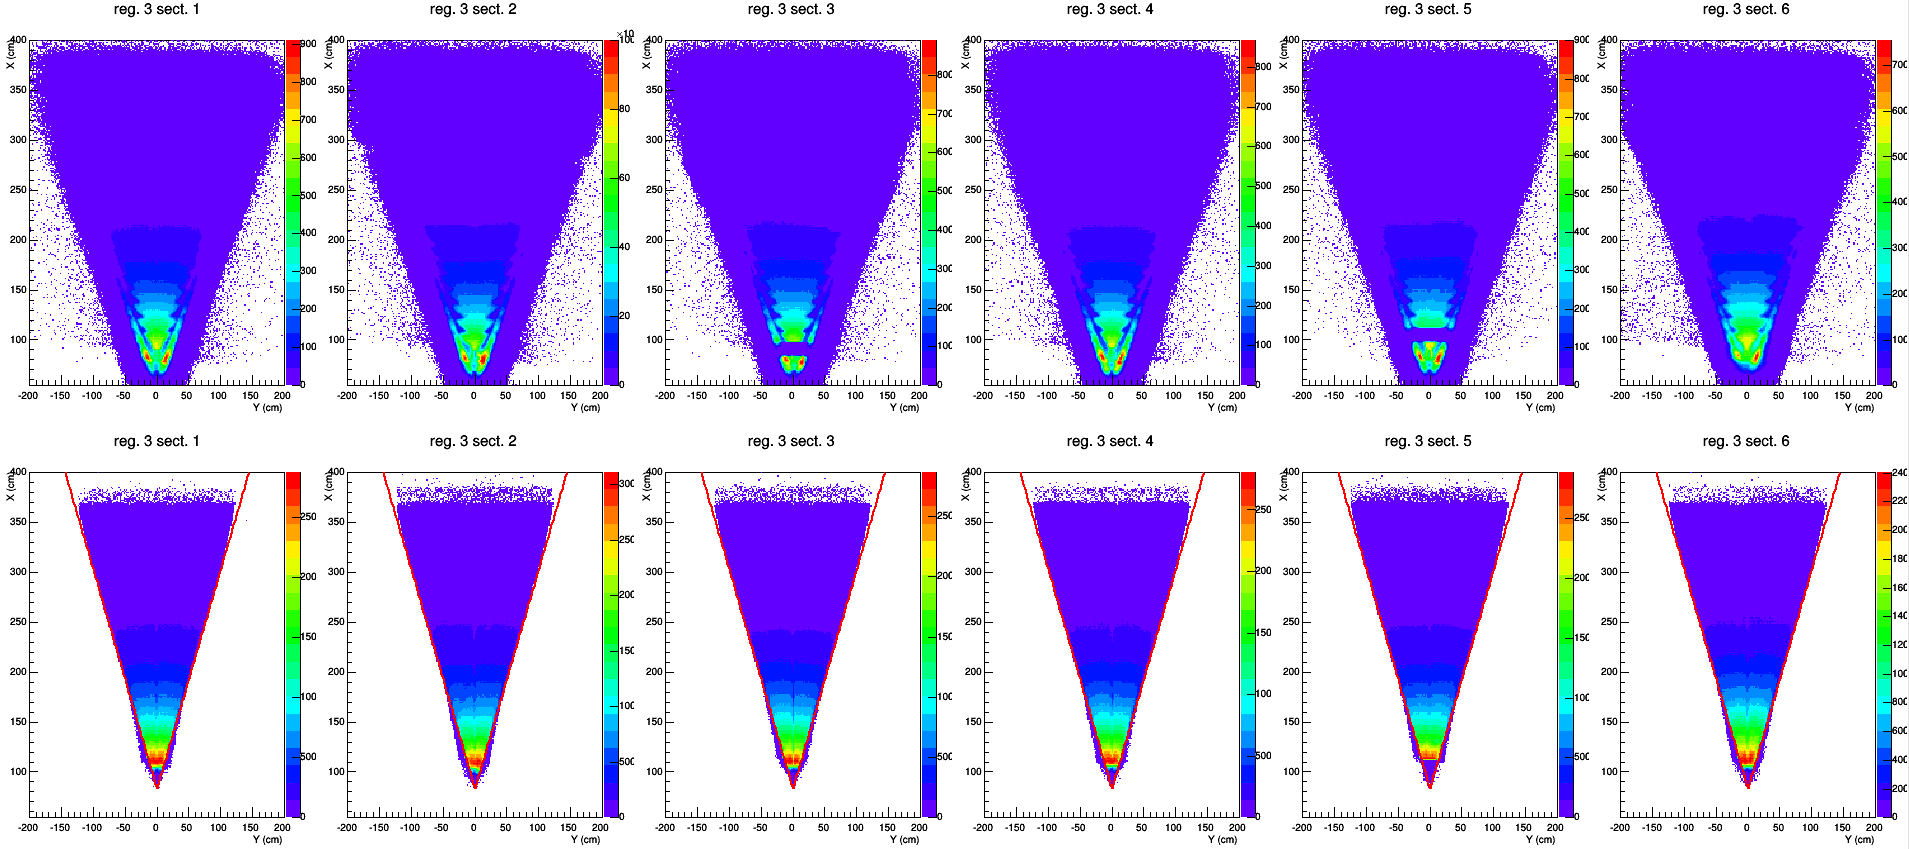
\includegraphics[width=8.5in]{figures/R3fid_c0c1_6sects.png}
\caption{The X vs Y position of tracks in region 3 of the DC for each sector. The top row shows results for all negative tracks and the bottom row shows results with all the other electron ID cuts applied. The cut applied here is shown with red lines.}
\label{fig:R3fid_c0c1_6sects}
\end{sidewaysfigure}
%

\section{z Vertex Correction and Cut}
\label{sec:zvertexCorrAndCut}
%
A cut is made on the z vertex to remove candidates that do not originate from the target.
The efficacy of the cut can be improved by first applying a vertex correction.
During reconstruction, a vertex $(x, y, z)$ is calculated for each charged track based on the intersection of the track with the midplane of the corresponding sector.
The midplane of a sector is the plane that divides the sector in half and contains the supposed beamline $(0, 0, z)$.
However, during the E1-f experiment the beam was not centered at $(x, y) = (0, 0)$, therefore a correction to the z vertex is applied.
Figure~\ref{fig:xyBeamOffset} shows the $(x, y)$ offset of the beam; events in this plot were selected from the aluminium foil located downstream from the target to fix the $z$ position.
The calculated value for the beam position is $(x, y) = (0.15 cm, -0.25 cm)$.

% the blank line above is on purpose to end the paragraph
\begin{figure}[htp]
\centering
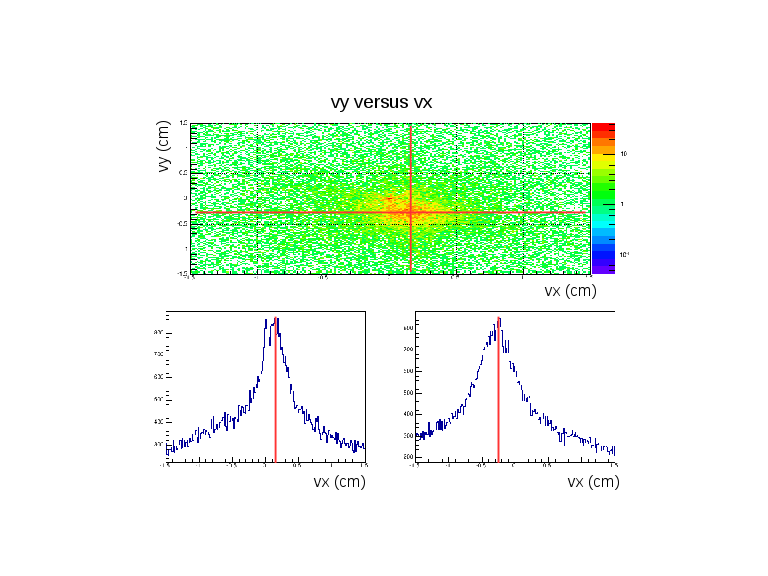
\includegraphics[width=6in, trim={1cm 1cm 1cm 1cm}, clip]{figures/xyBeamOffset.png}
\caption{Top: y vs x beam position for the E1-f run. Bottom left: x beam position for the E1-f run. Bottom right: y beam position for the E1-f run. The beam position is located at $x = 0.15 cm, y = -0.25 cm$ which is indicated by the red lines.}
\label{fig:xyBeamOffset}
\end{figure}
%
The z vertex is corrected by recalculating the intersection of the tracks with the midplanes after shifting the midplanes so that they contain the correct beamline $(0.15, -0.25, z)$.
The z vertex for electron candidates is plotted in figure~\ref{fig:corrVuncorrZvertex} before and after applying the correction.

% the blank line above is on purpose to end the paragraph
\begin{figure}[htp]
\centering
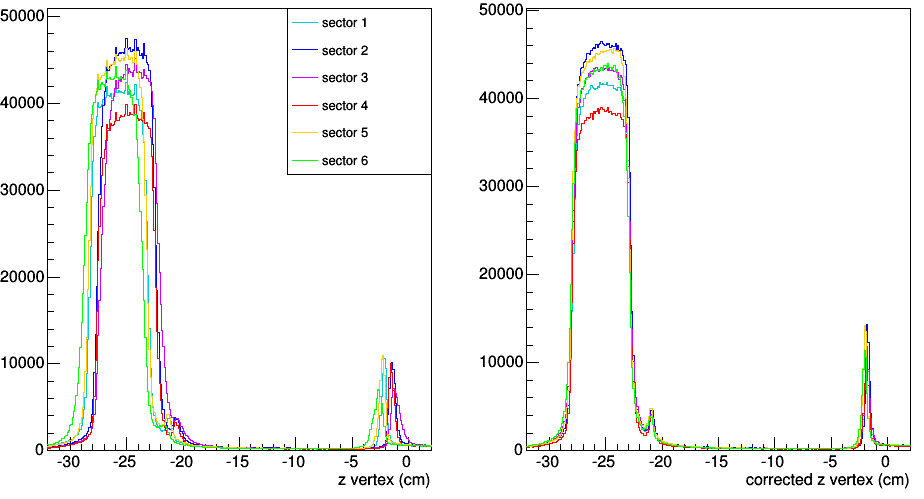
\includegraphics[width=6in]{figures/corrVuncorrZvertex.png}
\caption{Left: The z vertex for electron candidates for each sector. Right: The corrected z vertex for electron candidates for each sector. The two peaks near $-21 cm$ and $-2 cm$ are from aluminium foils placed there as reference points.}
\label{fig:corrVuncorrZvertex}
\end{figure}
%
The E1-f experiment was designed to have a $5 cm$ long target centered at $z = -25 cm$.
To have an even more precise location of the target, empty target runs are used to identify the positions of the target cell's entry and exit window (see figure~\ref{fig:emptyTargZ_integ6}).
The target cell's entry window was measured to be at $z = -27.7302 cm$ and the exit window was measured to be at $z = -22.6864 cm$; these values are used for the electron z vertex cut, which is shown in figure~\ref{fig:e_zvertexCut}.
%
\begin{figure}[htp]
\centering
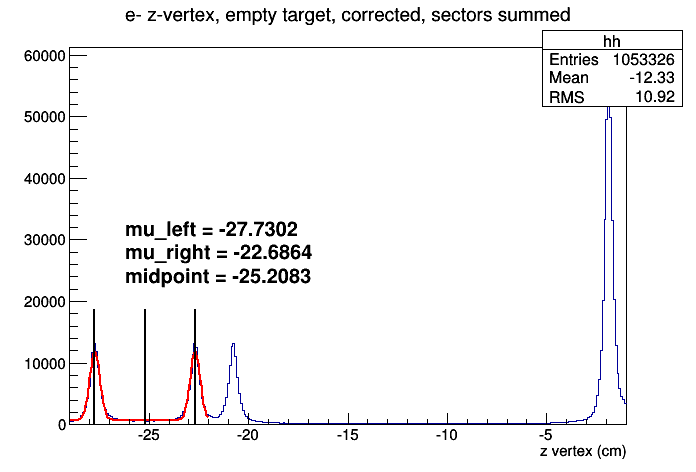
\includegraphics[width=4in]{figures/emptyTargZ_integ6.png}
\caption{The electron z vertex distribution for empty target runs. This data is used to identify the precise location of the target cell's entry and exit window. The two peaks near $-21 cm$ and $-2 cm$ are from aluminium foils placed there as reference points.}
\label{fig:emptyTargZ_integ6}
\end{figure}
%
\begin{figure}[htp]
\centering
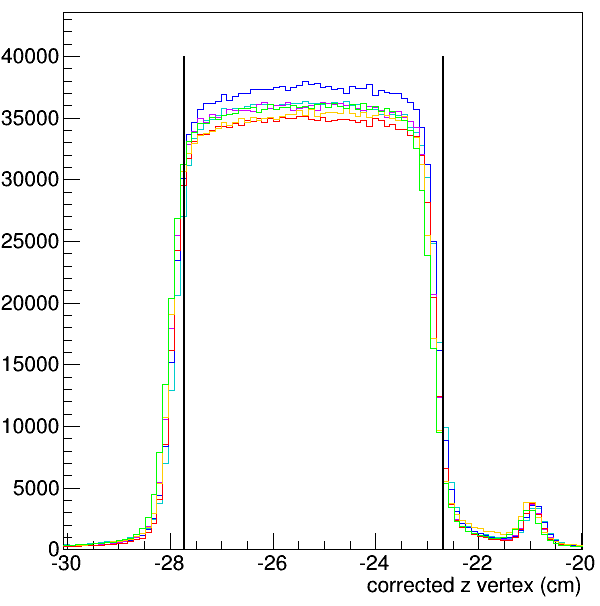
\includegraphics[width=3in]{figures/e_zvertexCut.png}
\caption{The corrected z vertex distribution for electrons candidates passing all the other electron ID cuts with this cut shown by black vertical lines. The peak near $-21 cm$ is from an aluminium foil placed there as a reference point.}
\label{fig:e_zvertexCut}
\end{figure}
%
\clearpage
